\section{Co-occurence based multimodal recommender}
\label{sec:design}
\tikzset{
  reco/.style={
    rectangle
  },
}

\begin{figure}
  \centering
  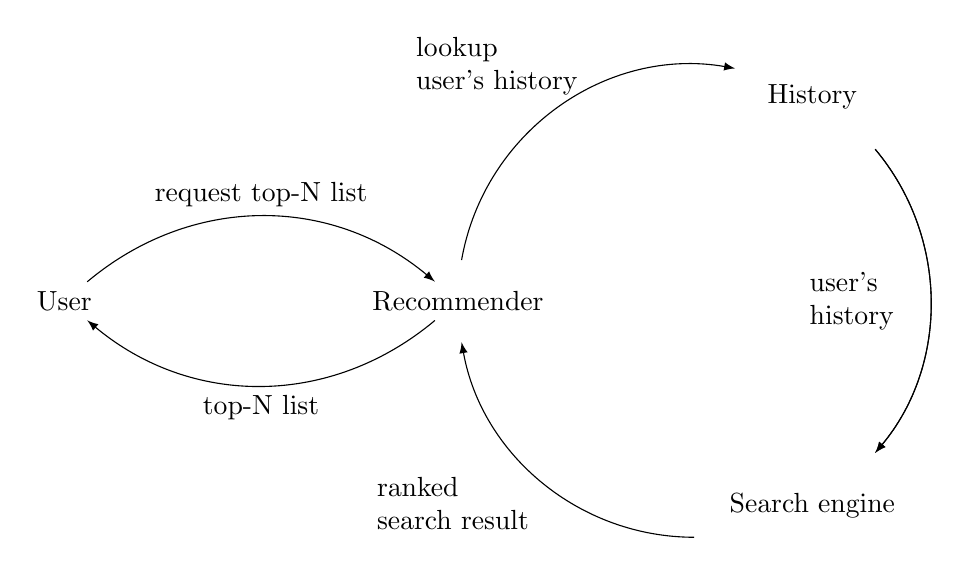
\begin{tikzpicture}[->, >=latex]
    \node[reco] (rec) at(180:3cm) {Recommender};
    \node (hist) at(60:3cm){History};
    \node (se) at(300:3cm){Search engine};
    \node (user) [left of=rec,node distance=5cm]{User};
    \node(x)[align=left] at(130:3.9cm){lookup\\ user's history};
    \node(x)[align=left] at(0:2cm){user's\\ history};
    \node(x)[align=left] at(220:4cm){ranked \\ search result};
    \draw[->, >=latex] (170:3cm) arc  (170:80:3cm);
    \draw[->, >=latex] (40:3cm)  arc (40:-40:3cm);
   \draw[->, >=latex] (270:3cm)  arc (270:190:3cm);
   \draw[->, >=latex] (40:3cm)  arc (40:-40:3cm);
   \path (user) edge[bend left=40] node[anchor=south,above]{request top-N list}(rec);
   \path (rec) edge[bend left=40] node[anchor=north,below]{top-N list}(user);
  \end{tikzpicture}
  \caption{Simplified dataflow diagram}
  \label{fig:topndataflow}
\end{figure}

The recommender we discuss will use past user behavior and metadata of items to compute the similarity between all items. Hence it is a hybrid recommender.
We use user \gls{coocc} of user- and tag-iteminteractions as a similarity metric among items.

Because search engine are a way of finding similar documents according to a query we can use a search engine to find similar items to the ones the user already exressed some interest.

The process of procucing a \gls{topn} can be divided into five steps. Figure \ref{fig:topndataflow} illustrates this process.

\begin{enumerate}
\item User requests a \gls{topn}.
\item The recommenders looks up items that appear in the recent user history.
\item The user's action history the recommender is send as a query to the search engine.
\item The search engine returns a ranked search result set of items according to the query.
\item The recommender removes item already known to the user and present him a \gls{topn}.
\end{enumerate}

The section first describes the used input data. Than we explain the process of computing \gls{topn} and how similarity between items is measured and how the computation is implemented. Next we describe the similarities of the top-N recommender task and a \gls{rankedretrieval} and how we extend the scoring function of the search engine in order to use \gls{coocc} similaty metric.

\subsection{Record user behavior}
\label{sec:inputdata}

\begin{figure}
  \centering
     \includegraphics[width=0.9\textwidth]{collectinginput}
  \caption{The user can like and tag movies with the web front end. The user actions are recorded by the web server.}
  \label{fig:gui}
\end{figure}

The \gls{rec} suggests items that are similar to the ones the user already liked in the past. In order to build a model for similarity we need to train the recommender with some data about the items.
This section will descibe the type of input data we use  in our demo application. The report will refer to this type of input data. 

Many collaborative filtering recommender engines use excplicit user ratings to train their model. Explicit user ratings of a user for an item are expressed by numbers (e.g. a rating is a number between 1 and 5). The use of explicit feedback has some drawbacks.
\begin{itemize}
\item Only a small subset of users will rate items. This leads to a model that is skewed against user who like to rate.
\item The majority of ratings are associated with a small fraction of the most popular items \cite{Anderson}. As a result it is less likely that unknown items show up in the \gls{topn}. This behavior is undesirable because the goal of the recommender is to present items the a user would not find on his own.
\end{itemize}

Corresponding to \cite{Dunning14} the best choice of input data is the collection past user actions on a website. The stored behavior of one user is called the user's \gls{history}. It shows what users actually do. Hence the input data should consist of recorded \glspl{useraction} (e.g. purchase, view, like, tag).

In our demo web application we record two different user actions:
\begin{description}
\item[like]  Users can express their positive feedback for a movie by clicking on a ``like'' button (the \gls{like} action is an explicit rating. We use it instead of a purchase or view action in order to keep the GUI simple).
\item[tag] User can \gls{tag} items. Every item can be associated with a list of \glspl{tag}.
\end{description}
The recorded like and tag action are later used to compute similarity between items.
Figure \ref{fig:gui} shows the simplistic user interface of our demo web app.

The web browser sends every user action to the web server. The web server provides a REST Web API that receives the \glspl{useraction} as HTTP \verb|Post| request and saves them to a sqlite3 \footnote{https://www.sqlite.org/} database.

In order to analyse the data later we want to retrieve the action history $h_u$ for a particular user $u$ for a defined action and a list of tags for every item. Hence we have to structure the data accordingly. Figure \ref{fig:er} shows the entity relationship diagram for the user actions \gls{like} and \gls{tag}

\tikzset{multi  attribute/.style={attribute ,double  distance=1.5pt}}
\tikzset{derived  attribute/.style={attribute ,dashed}}
\tikzset{total/.style={double  distance=1.5pt}}
\tikzset{every  entity/.style={draw=blue , fill=blue!20}}
\tikzset{every  attribute/.style={draw=yellow, fill=yellow!20, node distance=1.0cm}}
\tikzset{every  relationship/.style={draw=red, fill=red!20}}

\begin{figure}
\centering
\begin{tikzpicture}[node distance=2.0cm]
  \node[entity](user){user};
  \node[relationship](like)[above right of=user]{ like } edge (user);
  \node[attribute](date2)[above of=like]{ date } edge (like);
  \node[entity](item)[below right of=like]{item} edge (like);
  \node[relationship](tag)[below right of=user]{ tag } edge (user) edge (item);
  \node[attribute](text)[below right of=tag]{ text } edge (tag);
  \node[attribute](date1)[below left of=tag]{ date } edge (tag);
  \end{tikzpicture}
\caption{The data model allows us to retrieve the action history for every user. Like and tag form associations of user with item.}
\label{fig:er}
\end{figure}

It makes sense to start recording behavioral data month's before depoying the recommender engine because the recommender engine has to analyze the data and build a model of similarty among items in order to create personalized recommendations.


\subsection{How to compute the top-N recommendations list?}
\label{sec:problem}
This section gives a mathematical description of the top-N recommendation task and hence it describes the computations required to produce recommendations. The description refers to the \gls{rec}.

Suppose we have a metric to express similarity between two items as a numerical value and the magnitude of the value determines the strength of similarity. If we compute the similarity for every item pair in a set of $n$ items, we can represent the result in a matrix $M$. $M$ is a $n \times n$ matrix. Each row and each column contains the similarities between one particular item and all other items. $M$ is symetric across the diagonal because the similarity between $a$ and $b$ must be the same as between $b$ and $a$ (commutativity). The diagonal of $M$ contains the value for maximum similarity because this value represents the comparison of an item to itself. $M$ is called the \gls{indicatorm}. Equation \ref{eq:similaritymatrix} shows an example of an \gls{indicatorm} with 4 items.

\begin{equation}
  \label{eq:similaritymatrix}
M =\bordermatrix{~ & 1 & 2 & 3 & 4 \cr
 1 & 1  & 0.40 & 0.9 & 0.1 \cr
2 & 0.40 &1  & 0.9 & 0.1 \cr
 3& 0.9 & 0.9 &1  & 0.63 \cr
 4 & 0.1 & 0.1 & 0.63 &1  \cr}
\end{equation}
Further we represent a user action history for each user as vector $h_l$ of length $n$. $h_l$ contains an element for every item. The user's interactions with an item are represented as binary values in $h_l$. If the there is an interaction with an item in the history the value or the corresponding element is 1. Otherwise the value is 0. For example equation \ref{eq:history} shows a user's action history for the action ``like''. He has liked item 1 and 2.

\begin{equation}
\label{eq:history}
h_l =
\begin{pmatrix}
 1 \\
 1 \\
 0 \\
 0 \\
\end{pmatrix}
\end{equation}

To create a \gls{topn} for user $u$ we compute the matrix vector product of $M$ and $h_l$. The result $r$ is a vector of length $n$, that contains a value for every item. $r$ maps every item to a value that indicates how likely an item is of interest to user $u$. According to equation \ref{eq:recommendation} item 3 correspond to the best recommendation.

\begin{align}
  \label{eq:recommendation}
r_u &= M h_u 
&=
\begin{pmatrix}
  1  & 0.40 & 0.9 & 0.1 \\
 0.40 &1  & 0.9 & 0.1 \\
  0.9 & 0.9 &1  & 0.63 \\
  0.1 & 0.1 & 0.63 &1 \\  
\end{pmatrix} 
\begin{pmatrix}
 1 \\
 1 \\
 0 \\
 0 \\
\end{pmatrix}
&= 
\begin{pmatrix}
 1.4 \\
 1.4 \\
 1.8 \\
 0.2 \\
\end{pmatrix}
\end{align}

In order to create the complete \gls{topn} based on the vector $r$ we create a list of all item sorted by the values in $r$. Items with a high value appear first in the list. Then we remove all items from the list the user hasn't seen (the ones with zeros in $h_u$). In other words we return a ranked list of items. This list forms the \gls{topn}. In the example of equation \ref{eq:recommendation} the recommender would return item 3 followed by item 4. Item 1 and to are removed because the apear in the user's history.

\subsection{How to measure similarity among items?}
\label{sec:llr}

In the last section (\ref{sec:problem}) we use a matrix $M$ that contains similarity strengths among items. This section describes how $M$ is computed and why the \gls{llr} ratio of \glspl{coocc} is suitable for a recommender engine.

In order to compute the similarity between two items we count the \gls{coocc} among two items with respect to a particular user action and then compute the the \gls{llr} ratio of that \gls{coocc}.

\subsubsection{Co-occurrence}
\label{sec:cooccurence}

Co-occurrence in the context of a recommender system is the number of times a pair of items appear together in some user's action history or another item-interaction (e.g. tag-item). For instance, if there are 5 users who all liked items $A$ and $B$ then $A$ and $B$ co-occur 5 times. \Gls{coocc} indicates similarity. The more two items turn up together, the more related they probably are. We can count the \gls{coocc} of items with respect to any action or entity. For instance, we can count how many times two items are associated with the same tag or purchased by the same users.

\begin{figure}
\centering
\begin{tikzpicture}[node distance=40mm,
data/.style={
rectangle,
draw,
thin,
minimum height=3.5em
},
to/.style={->,>=stealth',shorten >=1pt,semithick,font=\footnotesize},
]
\node (hist) [data, align=left] {User actions\\history};
\node (co) [data,right of=hist,align=left] {Co-occurence};
\node (in) [data,right of=co,align=left] {LLR\\indicator\\matrix};
\draw[to] (hist) -- (co);
\draw[to] (co) -- (in);
\end{tikzpicture}
\caption{To compute the indicator matrix we first count the co-occurrences of items and then we compute the log-likelihood strengths of the \glspl{coocc}.}
\label{fig:llrworkflow}
\end{figure}

\subsubsection{Log-likelihood ratio}
\label{sec:llrs}

\Gls{llr} is a probabilistic measure of the importance of a \gls{coocc}. The \gls{llr} similarity  is the probability that two users share the same items because the items are similar and not due to chance. It finds important \glspl{coocc} and filters out the coincidental. Hence it avoids that the result is skewed against popular items \cite{Dunning93}. Compared to the Jaccard coefficient \cite{Hartung} the log-likelihood-based similarity computes higher similarities for anomalous co-occurrences than for items that occur in every user history. For a detailed explanation of the math involved see \cite{Dunning93}. 

According to \cite{Dunning14} using the \gls{llr} ratio of the \gls{coocc} has several advantages.
\begin{itemize}
\item It yields good results for data that only captures the interaction and no explicit numerical \glspl{preference} value \cite{Dunning93}.
\item The similarity is not skewed against popular items.
\item We can use distributed MapReduce based algorithms to compute the \glspl{coocc}. Hence the computation of the \gls{llr} similarity is \gls{scalable}.
\end{itemize}

\subsubsection{Example}
\label{sec:llrexample}

We describe the log-likelihood based similarity with a small example data set. Suppose we analyze the user action history for the action ``like'' given in table \ref{tbl:llr1}. 
Table \ref{tbl:llr1} shows the likes of four users for five items. The items are represented with integers 1-4 and the users with integers 101 - 104  (see appendix listing \ref{lst:sampledata} for raw web log).
In the example data set of table \ref{tbl:llr1} the items 1 and 2 are similar because three users liked both of them.

We compute the \gls{indicatorm} in two steps as shown in figure \ref{fig:llrworkflow}.
\begin{enumerate}
\item Count \glspl{coocc}
\item Compute \gls{llr} of \glspl{coocc}
\end{enumerate}

\begin{table}
\begin{center}
\begin{tabular}{rllll}
 & 101 & 102 & 103 & 104\\
1 & x & x & x &  \\
2 & x &   & x & x\\
3 & x & x & x &  \\
4 &   & x & x & x\\
5 & x & x & x & x\\
\end{tabular}
\end{center}
\caption{Example data set. The columns represent the user interaction with an item. Items are named 1 - 4 and users 101 - 104}
\label{tbl:llr1}
\end{table}

In order to get the similarities between all items we count the \gls{coocc} of ``\glspl{like}'' for all item pairs. This leads to the $5 \times 5$ \gls{indicatorm} $C$ shown in equation \ref{eq:coocm}. The rows and the columns are items. $C$ is a similarity comparison of every row of table \ref{tbl:llr1} to every other row.

\begin{equation}
  \label{eq:coocm}
C =\bordermatrix{~ & 1 & 2 & 3 & 4 & 5 \cr
1 & 4 & 2 & 3 & 2 & 3 \cr
2 & 2 & 3 & 2 & 1 & 3 \cr
3 & 3 & 2 & 3 & 2 & 3 \cr
4 & 2 & 1 & 2 & 3 & 3 \cr
5 & 3 & 3 & 3 & 3 & 4 \cr}
\end{equation}

In the next step we compute the \gls{llr} ratio strength of the \glspl{coocc} for every item pair. This will again produce a $5 \times 5$ \gls{indicatorm}. Equation \ref{eq:coocm1} shows the \gls{indicatorm} for the sample data set from table \ref{tbl:llr1}.

\begin{equation}
  \label{eq:coocm1}
L =\bordermatrix{~ & 1 & 2 & 3 & 4 & 5 \cr
1 &   & 0.40 & 0.81 & 0.63 & 0 \cr
2 & 0.40 &  & 0.40 & 0.63 & 0 \cr
3 & 0.81 & 0.40 &  & 0.63 & 0 \cr
4 & 0.63 & 0.63 & 0.63 &  & 0 \cr
5 & 0 & 0 & 0 & 0 & \cr
}
\end{equation}

Although item 5 shares all users with item 1 and 3, the log-likelihood ratio is 0 because every user purchased item 5. The goal of collaborative filtering is to show the user items he would not find by himself. Item 5 is popular and a user will probably discover it by looking up a list of items sorted by popularity (this is a form of non-personalized recommendation). Hence Item 5 is not a valuable personal recommendation because we could extract it without a recommender. For this reason the \gls{llr} is suitable similarity metric for a recommender engine.

\subsubsection{Log-likelihood similarity implementation}
\label{sec:llrimpl}

Apache Mahout provides an implementation of log-likelihood similarity with the class \verb|LogLikelihoodSimilarity|. Unfortunately the LogLikelihoodSimilarity is a non-distributed implementation. It would take too long to calculate the indicator matrix for a data set with over 10 million items and we would have difficulties to load all data into the memory. 

The computation of the \gls{coocc} of every item pair can be distributed and run in parallel by applying the MapReduce programming model as follows:
\begin{description}
\item[Map] Determine all \glspl{coocc} for one user's history and yield a pair of items for each \gls{coocc}
\item[Reduce] For each item collect all corresponding item pairs of the map phase and count all \glspl{coocc} and yield a vector with all items and the corresponding \gls{coocc}.
\end{description}

This task can run in parallel on different nodes on a cluster computer framework, such as Apache Spark. Hence the computation of the \gls{indicatorm} is \gls{scalable}.
In order to compute the \gls{llr} similarity distributed on a Spark cluster, Apache Mahout provides the \verb|spark-item-| \verb|similarity| job. 
\verb|spark-itemsimilarity| is a command line job and we can start it from the Mahout shell.
\begin{verbatim}
./mahout spark-itemsimilarity --input $infile --output $outfile
\end{verbatim}
The job connects to the Spark cluster instance defined by the environment variable \verb|MASTER| and computes the \gls{indicatorm} in parallel. With the \verb|spark-itemsimilarity| job the indicator matrix can be computed in $O(n)$ \cite{Schelter}. 
The input text file contains a row for every user-item interaction. They have to be in the following format:
\begin{verbatim}
userID, action, itemID
\end{verbatim}
The output will be a text file that represents the indicator matrix as sparse vectors for every item. For every item we get the similarities to all other items.
\begin{verbatim}
itemID1<tab>itemID2:similarityvalue<space>itemID3:simvalue...
\end{verbatim}

In our demo application we have written a Python script to fetch the data from the sqlite3 database and transform to the Spark input format.


\subsection{Using more than one type of behavior}
\label{sec:multimodal}

Most collaborative filtering algorithms use only explicit or implicit ratings to compute similarity.
But we can improve the performance of the recommender engine by using multiple types of user actions. In addition to likes we could use tag-associations to compute the similariy. In table \ref{tbl:llr} we count co-occurence of items in a user's like-action history. Instead of the action history we could use tags that are associated width items. We count the co-occurence of each items associated with a tag.

Suppose we compute a \gls{indicatorm} based on likes $M_l$ and one based on tag associations $M_t$. An $h_l$ is a user's history of ``likes'' and $h_t$ is the user's tag history. Then we can compute the recommendation vector (see equation \ref{eq:recommendation}) $r$ with

\begin{equation}
  \label{eq:multi}
  r = h_l M_l + h_t M_t
\end{equation}

In our demo web application we use ``likes'' and tags but virtually all user actions can be used to improve the recommendation.

\subsection{Why can we use a search engine to produce \gls{topn}?}
\label{sec:relation}

The \gls{rec} uses a search engine to produce a \gls{topn}. We can deploy a search engine in order to provide recommendations because there are similarities between the computation of the \gls{topnt} and the retrieval of a ranked search result set.
 This section explains why the deployment of a search engine is suitable for the top-N recommendation task.

\subsubsection{Ranked retrieval}
A search engine enables user to search a collection of documents for specified keywords in a query. A document contains several \glspl{field}. A \gls{field} contains a sequence of terms or meta data about the document. A user can search for documents that contain keywords only in specific fields. The search engine returns a sorted set of documents that match the query. The result set is sorted by relevancy. The top documents are the most relevant to the query. This process is called \gls{rankedretrieval}. The search engine does this by calculating a similarity score between each document and the query and then sorts the result by this score. The score indicates the strength of the match against the query. This is one of the main use cases where search engines shine compared to relational databases. There a row either matches a query or it does not. 

\subsubsection{Vector space model}
One way to calculate the similarity between a query $q$ and a document $d$ is to use the vector space model.
In the vector space model each document $d$ and the query $q$ are represented as vectors $\vec{v}(d)$ and $\vec{v}(q)$. The vector contains an element for each term. It maps every term $t$ of the collection to a tf-idf weight. tf-idf reflects how important a term is to a document in the collection (see \cite{Manning} for a detailed description). 
The similarity score between two items is equal to the dot product.
\begin{equation}
  \label{eq:score}
  \text{score}(d,q) = \vec{v}(d) \cdot \vec{v}(q)
\end{equation}
In order to create a ranked result set for a query $q$ the search engine computes $\text{score}(d,q)$ for all documents in the collection. We can form a matrix $C$ with the document vectors as rows. The process of scoring all document can be written as matrix vector multiplication of $C$ and $q$. 
\begin{equation}
  \label{eq:ser}
  r = C q
\end{equation}
$r$ maps every document to a relevancy score.
This is similar to the computation of the \gls{topn} $r_u = M h_u$  described in section \ref{sec:problem}. The search engine returns documents with fields who's vector representation $\vec{d}$ is similar to the query vector $\vec{q}$. The recommender returns items that are similar to the items in the user's action history $h_u$. If we can map items to documents and the user's action history to a query we can use an existing search engine for the top-N recommendation task. This is desirable because search engines like Apache Solr are optimized for ranked retrieval and they are able to process big data at scale. 

\subsubsection{How to map documents to items}
\label{sec:mapping}

\begin{lstlisting}[caption={Item meta data and similar items are stored in Solr.},label={lst:solrdoc}]
{
    id: 1,
    title: Toy Story,
    tags:Pixar animation fantasy,
    likeindicator: 1688 1834 3893 4366 6281 33162,
    tagindicator: 10 33 41 54 55 59 66 67 72 73 80
    _version_: 1505056335358591000
}
\end{lstlisting}

The result of the search should contain a list of items. Hence we index items instead of documents.

Instead of finding documents that contain the keywords of the query in a field we want to find items that are similar to the items in the user's action history. We will first discuss a simple approach. 

For item $i$ we store all items whose \gls{llr} ratio (described in section \ref{sec:llrs} to $i$ is above a defined threshold in a separate field. For every type of user action we create such a field. These fields are called \glspl{indicatorfield}. 

Figure \ref{lst:solrdoc} shows an example entry of a movie item formatted in JSON. The indicator fields \verb|likeindicator| and \verb|tagindicator| contain movie ID's of similar movies. In addition to the indicator fields, the entry contains meta data about the item. These fields can be used to retrieve items by meta data, such as title or genre.

We query the search engine with items from the user's action history $h$. The search engine will transform the items in the query to the corresponding document vector. Table \ref{tbl:comparison} shows the mapping.

This way the search engine computes a higher score for documents that contain the items in $h$ also in their indicator fields. The more items the query $h$ and an indicator field of $i$ have in common the higher the similarity score for a document. Hence the search engine returns similar items the user already liked. In addition the tf-idf weights of the document vectors will mitigate popular items. The drawback of this simplified approach is that it does not account for different \gls{llr} similiarity values betwenn items above threshold. They are ignored.

 We want to have some way to include the \gls{llr} ratios of the \gls{indicatorm} $M$ to boost items that have a high similarity to the item represented by the document. In order to include the similarity metric among items described in section \ref{sec:llr} we have to weight the tf-idf values in the document vector with the \gls{llr} ratios. This is the reason why we can't use a search engine out of the box without extending it's scoring function. 

\begin{table}
\begin{center}
\begin{tabular}{lll}
 search engine & \gls{rec}\\ \hline
  document & item\\ 
 field & indicatorfield \\
 term & item (item id)    \\
 query & user's action history \\
payload & LLR similarity \\
\end{tabular}
\end{center}
\caption{We can map document, fields, term and query to the recommender equivalents.}
\label{tbl:comparison}
\end{table}

\subsubsection{Emulate different recommender strategies}

Note that we can emulate different recommendation engines by using different queries.
\begin{itemize}
\item If the query is composed with the user's action history we use collaborative filtering with an \gls{itembased} approach.
\item We can use a single item $i$ as query and get back all similar items. For instance, a top-N list of items retrieved with this query can be placed on a description page of item $i$ with the title ``Customers Who Liked This Item Also Liked''. This is a non-personalized approach.
\item We can use user profile information in the query. If the user profile contains information about the user's favorite movie genre or favorite director and the search engine has indexed the corresponding meta data we can search for items that match the user' profile. This would be a content based approach.
\end{itemize}

\subsubsection{Implementation}
\label{sec:solrimpl}
We deploy the search engine Apache Solr in our demo webapplication. Simply put, Solr is a Web API for Apache Lucene, an open source information retrieval software library. 

In order to use the precomputed \gls{llr} ratios of the \glspl{coocc} we need a way to store them per term and per document. Lucene provides this functionality with the \emph{playloads} feature. Payloads enable an application to store an arbitrary byte array for every term during indexing \cite{McCandless}.

Unfortunatly the feature is only implemented in Lucence, not in Solr. But we can extend Solr to use the Java classes that deal with payloads.

First we need to define a new fieldtype in the schema.xml of our Solr configuration. Fields of this type contain terms with an added payload.
To index the similarity value we define a custom fieltype that uses Lucene's DelimitedPayloadTokenFilter to extract a payload from every term. 

\begin{lstlisting}[caption={Fieldtype definition for field with payload.}]
<fieldtype name="payloads" class="solr.TextField" >
 <analyzer>
  <tokenizer class="solr.WhitespaceTokenizerFactory"/>
   <filter class="DelimitedPayloadTokenFilterFactory" />
 </analyzer>
</fieldtype>
\end{lstlisting}
The default delimiter is the pipe symbol. With this fieldtype we can add payloads to terms in document be attaching a number to the term string.
\begin{verbatim}
23|0.9
\end{verbatim}
In this example \verb|23| is an item-id and \verb|0.9| is the similiarity value to the corresponding item.

After we stored the payload within the index we need a way to score a document match according the payload.
Solr uses per default the vector space model to compute the score between a document $d$ and a query $q$. It only considers terms $t$ that appear in the query $q$. The tf-idf weight is multiplied by a boosting factor for a term $t$ \cite{grainger}.  
\begin{equation}
\label{eq:solrsim}
\text{score}(q,d) = \sum_{t \in q} \text{tf-idf}(t,d) \cdot \text{boost}(t)
\end{equation}

In order to use the payload values in the ranked retrieval process we have to extend Solr with our own Query Component. 

We can add a custom Query Component by implementing a \verb|QParserPlugin|. The implementation just returns the \verb|PayloadTermQuery|. \verb|PayloadTermQuery| matches all documents containing the specifed term and than applies a scoring factor based on the payload that is stored with each term.

In addition we have to override the method \verb|scorePayload| of the \\ \verb|DefaultSimilarity| class. \verb|PayloadTermQuery| will call \verb|scorePayload| to determine the payload of an item and then it multiplies the td-idf weights with the corresponding payload. We have to tell Solr to use our custom Query Component and the new \verb|PayloadSimilarity| by adding the following entries to the solrconfig.xml.

\begin{lstlisting}
<similarity class="ch.hsr.solrpayload.PayloadSimilarityFactory">
<queryParser name="payloadparser" 
   class="ch.hsr.solrpayload.PayloadParser" />
\end{lstlisting}
  
Solr will load the implementations from it's \verb|lib| directory if we package them Java jar archive.

\begin{figure}
  \centering
\begin{tikzpicture}
  \begin{axis}[
    title=evaluation of LLR threshold,
    xlabel=threshold,
    ylabel=Precision/Recall,
    width=10cm,
    ]
\addplot table {thresholdp.dat};
\addplot table {thresholdr.dat};

  \end{axis}
\end{tikzpicture}
\caption{The precision and recall at 10 for the MovieLens data set is measured as a function of the similarity threshold. Items with a small similarity value do not contribute to the performance. The best performance is archieved by only adding items with a \gls{llr} ratio above 0.9.}
\label{fig:threshold}
\end{figure}

In our demo web application we only add items above a given \gls{llr} ratio threshold to the index of the search engine. If we add items with a small similarity to the indicator fields the precision and recall decline. The evaluation in figure \ref{fig:threshold}shows that the we archieve the best performance with a threshold of 0.9.

An alternative to the use of payloads is to ignore similarities values once we removed the item below threshold from the index. In that case the scoring of a document only depends on the tf-idf weight. Only add items above a threshold to the indicator fields. This approach is easier to deploy but it doesn't account for different similaries. 

\section{Integration}
\label{sec:integration}

This section will describe the integration of the \gls{rec}. In section will describe how we integrate components described in section \ref{sec:design.}

The recommender discussed in this report has to parts.
\begin{description}
\item[Compute similarities] In this part the user action are analised in order to compute the similarities of items. The similiarities are stored as indicators in Apache Solr.
\item[Generate personalized recommendations] A systems formats a list of recommended items.
\end{description}


\subsubsection{Retrieve recommendation}

In order to produce recommendations we compose a Solr query from the user history. The user history is stored in the web log. The web server sends this query to Solr. Solr responds with a ranked result set. The web server then formats the response from Solr and sends a list of recommended items to the user.

\begin{figure}
\centering
\begin{tikzpicture}[node distance=20mm,
data/.style={
rectangle,
draw,
thin,
minimum height=3.5em
},
to/.style={->,>=stealth',shorten >=1pt,semithick,font=\footnotesize},]

\node (web) [data] {Web server};
\node (log) [data,below of = web, align=left] {User actions\\log file};
\node (browser) [data,left of=web,node distance=50mm] {Webbrowser};
\node (solr) [data,right of=web,node distance=50mm] {Search engine};
\draw[to] (web) -- (log);
\draw[to] (browser) -- node[midway,above] {user actions} (web);
\end{tikzpicture}
\caption{The web server sends this query to Solr. Solr responds with a ranked result set.}
\end{figure}

\verb|updatesearchengine| will index all movies in Solr.

Solr is used in the offline and the online part of the recommendation engine.

The items and their corresponding similarity indicators from the Apache Spark job are stored with Apache Solr. 

We store all items as documents in Solr. The documents contain the metadata like (title, genre, tags, etc). In addidtion we populate a filed for every indicator with the similar item ID's discovered with the coocuccence similartiy from section \ref{sec:llr}.

In order to build a recommender using a search engine we store the output of the co-occurence analysis in Solr. The search engine actually delivers the recommendations to our users.

\subsection{Parameters}
\label{sec:parameters}

This section descripes the paratemter of the recommender discussed in this report.
\begin{description}
\item[similarity threshold] We have to define a threshold to separate similar items occording to the LLR similarity from the rest (e.g. 0.5).
\item[user history to consider] We retrieve recommendations with a part of the user history. We have to define the number of log entries to consider.
\end{description}

\subsection{Two-parts design}

The recommender described in this article is divided in two parts.
\begin{itemize}
\item Computation of simililarity and the update of the text search engine is done offline, ahead of time.
\item Recommendations are generated instantly by quering the text search engine using rescents actions of the user.
\end{itemize}
